\documentclass[aspectratio=169,12pt]{beamer}

% Theme and colors
\usetheme{Madrid}
\usecolortheme{whale}
\setbeamertemplate{navigation symbols}{}
\setbeamertemplate{footline}[frame number]

% Packages
\usepackage{amsmath,amssymb}
\usepackage{graphicx}
\usepackage{tikz}
\usetikzlibrary{shapes,arrows,positioning,calc,matrix}
\usepackage{booktabs}
\usepackage{array}
\usepackage{multirow}
\usepackage{xcolor}
\usepackage{hyperref}

% Custom colors
\definecolor{codegreen}{rgb}{0,0.6,0}
\definecolor{codepurple}{rgb}{0.58,0,0.82}
\definecolor{darkblue}{rgb}{0,0,0.7}

% Title information
\title[Cloud Computing for Multimedia]{Cloud Computing for Multimedia Services}
\subtitle{Part III --- Multimedia Communications and Networking}
\author[Mahesh C]{\textbf{Mahesh C}\\FISAT}
\institute{Federal Institute of Science and Technology (FISAT)\\Multimedia Technology Class}
\date{\today}

\begin{document}

% Title slide
\begin{frame}
    \titlepage
    \begin{center}
        \small Based on: Li, Drew \& Liu, \textit{Fundamentals of Multimedia}, Chapter 19
    \end{center}
\end{frame}

% Outline
\begin{frame}{Outline}
    \tableofcontents
\end{frame}


%==============================================================================
\section{Cloud Computing Overview}
%==============================================================================

\begin{frame}{What is Cloud Computing?}
    \begin{block}{NIST Definition (Mell \& Grance, 2011)}
        Cloud computing is a model for enabling ubiquitous, convenient, on-demand network access to a shared pool of configurable computing resources (e.g., networks, servers, storage, applications) that can be rapidly provisioned and released with minimal management effort.
    \end{block}
    
    \vspace{0.3cm}
    \textbf{Five Essential Characteristics:}
    \begin{enumerate}
        \item \textbf{On-demand self-service} --- provision resources automatically
        \item \textbf{Broad network access} --- available over the network
        \item \textbf{Resource pooling} --- shared among multiple users
        \item \textbf{Rapid elasticity} --- scale up or down quickly
        \item \textbf{Measured service} --- pay for what you use
    \end{enumerate}
\end{frame}

\begin{frame}{Cloud Service Models}
    \begin{center}
        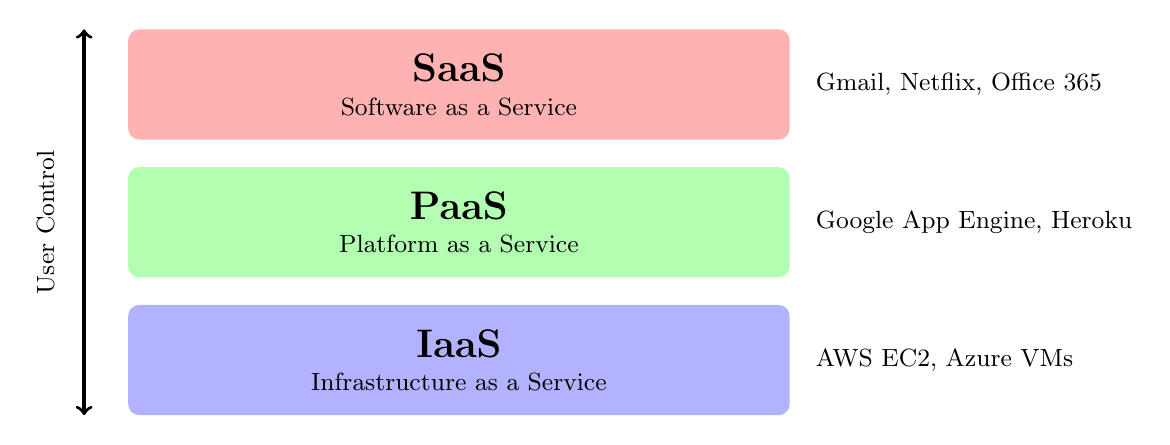
\begin{tikzpicture}[scale=0.7]
            % SaaS
            \fill[red!30, rounded corners] (0,6) rectangle (12,8);
            \node at (6,7.3) {\Large\textbf{SaaS}};
            \node at (6,6.6) {\small Software as a Service};
            \node[right] at (12.3,7) {\small Gmail, Netflix, Office 365};
            
            % PaaS
            \fill[green!30, rounded corners] (0,3.5) rectangle (12,5.5);
            \node at (6,4.8) {\Large\textbf{PaaS}};
            \node at (6,4.1) {\small Platform as a Service};
            \node[right] at (12.3,4.5) {\small Google App Engine, Heroku};
            
            % IaaS
            \fill[blue!30, rounded corners] (0,1) rectangle (12,3);
            \node at (6,2.3) {\Large\textbf{IaaS}};
            \node at (6,1.6) {\small Infrastructure as a Service};
            \node[right] at (12.3,2) {\small AWS EC2, Azure VMs};
            
            % Arrow
            \draw[<->, very thick] (-0.8,1) -- (-0.8,8);
            \node[rotate=90] at (-1.5,4.5) {\small User Control};
        \end{tikzpicture}
    \end{center}
\end{frame}

\begin{frame}{Cloud Deployment Models}
    \begin{columns}
        \begin{column}{0.5\textwidth}
            \textbf{Public Cloud}
            \begin{itemize}
                \item Open to general public
                \item Owned by cloud provider
                \item Pay-per-use pricing
                \item Examples: AWS, Azure, GCP
            \end{itemize}
            
            \vspace{0.3cm}
            \textbf{Private Cloud}
            \begin{itemize}
                \item Exclusive to one organization
                \item Higher security and control
                \item Higher cost
                \item Example: Company data center
            \end{itemize}
        \end{column}
        \begin{column}{0.5\textwidth}
            \textbf{Hybrid Cloud}
            \begin{itemize}
                \item Mix of public and private
                \item Sensitive data stays private
                \item Burst to public for peak loads
                \item Most enterprises use this
            \end{itemize}
            
            \vspace{0.3cm}
            \textbf{Community Cloud}
            \begin{itemize}
                \item Shared by organizations with common concerns
                \item Example: Government agencies
                \item Shared cost and compliance
            \end{itemize}
        \end{column}
    \end{columns}
\end{frame}

\begin{frame}{Why Cloud Matters for Multimedia}
    \textbf{Multimedia is resource-hungry:}
    
    \begin{columns}
        \begin{column}{0.5\textwidth}
            \textbf{Compute demands:}
            \begin{itemize}
                \item Video transcoding (CPU/GPU intensive)
                \item Image recognition and AI
                \item Real-time rendering
                \item Audio/video processing
            \end{itemize}
            
            \vspace{0.3cm}
            \textbf{Storage demands:}
            \begin{itemize}
                \item Netflix library: 15,000+ titles
                \item YouTube: 500+ hours uploaded/min
                \item Instagram: 100M+ photos/day
            \end{itemize}
        \end{column}
        \begin{column}{0.5\textwidth}
            \textbf{Bandwidth demands:}
            \begin{itemize}
                \item 4K video: 25 Mbps per stream
                \item Global distribution needed
                \item Low latency required
            \end{itemize}
            
            \vspace{0.3cm}
            \begin{alertblock}{The Cloud Solution}
                Cloud provides elastic compute, massive storage, and global distribution --- exactly what multimedia needs!
            \end{alertblock}
        \end{column}
    \end{columns}
\end{frame}

%==============================================================================
\section{Multimedia Cloud Computing}
%==============================================================================

\begin{frame}{Multimedia Cloud Computing (Zhu et al., 2011)}
    \begin{block}{Definition}
        Multimedia Cloud Computing (MCC) refers to the use of cloud computing infrastructure to provide multimedia services including storage, processing, delivery, and consumption of multimedia content.
    \end{block}
    
    \vspace{0.3cm}
    \begin{center}
        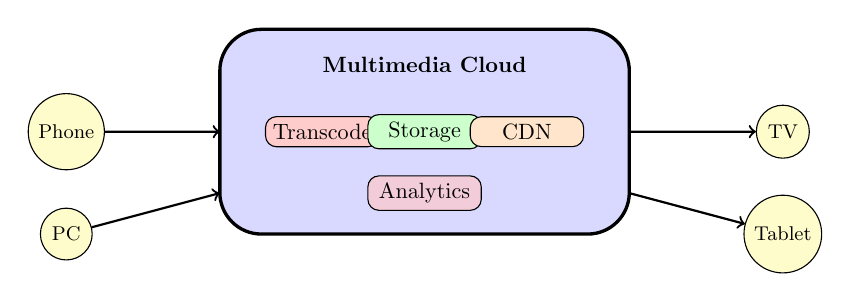
\begin{tikzpicture}[scale=0.65, every node/.style={scale=0.8}]
            % Cloud
            \draw[fill=blue!15, very thick, rounded corners=15pt] (3,3) rectangle (11,7);
            \node at (7,6.3) {\textbf{Multimedia Cloud}};
            
            % Services inside cloud
            \node[draw, fill=red!20, rounded corners, minimum width=1.8cm] at (5,5) {Transcode};
            \node[draw, fill=green!20, rounded corners, minimum width=1.8cm] at (7,5) {Storage};
            \node[draw, fill=orange!20, rounded corners, minimum width=1.8cm] at (9,5) {CDN};
            \node[draw, fill=purple!20, rounded corners, minimum width=1.8cm] at (7,3.8) {Analytics};
            
            % Users
            \node[draw, fill=yellow!20, circle] (u1) at (0,5) {\small Phone};
            \node[draw, fill=yellow!20, circle] (u2) at (0,3) {\small PC};
            \node[draw, fill=yellow!20, circle] (u3) at (14,5) {\small TV};
            \node[draw, fill=yellow!20, circle] (u4) at (14,3) {\small Tablet};
            
            % Connections
            \draw[->, thick] (u1) -- (3,5);
            \draw[->, thick] (u2) -- (3,3.8);
            \draw[->, thick] (11,5) -- (u3);
            \draw[->, thick] (11,3.8) -- (u4);
        \end{tikzpicture}
    \end{center}
\end{frame}

\begin{frame}{Key Components of Multimedia Cloud}
    \textbf{Four pillars of multimedia cloud computing:}
    
    \vspace{0.3cm}
    \begin{columns}
        \begin{column}{0.5\textwidth}
            \textbf{1. Cloud Storage}
            \begin{itemize}
                \item Store massive media libraries
                \item Redundancy and reliability
                \item Geo-distributed replicas
                \item Cost-effective scaling
            \end{itemize}
            
            \vspace{0.3cm}
            \textbf{2. Cloud Processing}
            \begin{itemize}
                \item Video transcoding at scale
                \item Image/audio processing
                \item AI-based content analysis
                \item Parallel processing
            \end{itemize}
        \end{column}
        \begin{column}{0.5\textwidth}
            \textbf{3. Cloud Delivery (CDN)}
            \begin{itemize}
                \item Content Distribution Networks
                \item Edge caching near users
                \item Adaptive bitrate streaming
                \item Low-latency delivery
            \end{itemize}
            
            \vspace{0.3cm}
            \textbf{4. Cloud Analytics}
            \begin{itemize}
                \item User behavior analysis
                \item Content recommendation
                \item Quality of Experience (QoE)
                \item Network optimization
            \end{itemize}
        \end{column}
    \end{columns}
\end{frame}

\begin{frame}{Challenges in Multimedia Cloud Computing}
    \begin{columns}
        \begin{column}{0.5\textwidth}
            \textbf{Technical Challenges:}
            \begin{itemize}
                \item \textbf{Latency:} Real-time multimedia needs low delay ($<$150 ms for interactive)
                \item \textbf{Bandwidth:} Video consumes enormous bandwidth
                \item \textbf{Heterogeneity:} Diverse devices, screens, codecs
                \item \textbf{QoS guarantees:} Cloud is shared; multimedia needs consistent quality
            \end{itemize}
        \end{column}
        \begin{column}{0.5\textwidth}
            \textbf{Economic Challenges:}
            \begin{itemize}
                \item \textbf{Cost:} Transcoding and storage are expensive at scale
                \item \textbf{Pricing models:} Pay-per-use vs reserved capacity
                \item \textbf{Vendor lock-in:} Difficult to switch providers
            \end{itemize}
            
            \vspace{0.3cm}
            \begin{block}{Key Tradeoff}
                \textbf{Quality vs Cost vs Latency}
                
                You can optimize two, but the third suffers!
            \end{block}
        \end{column}
    \end{columns}
\end{frame}


%==============================================================================
\section{Cloud-Assisted Media Sharing}
%==============================================================================

\begin{frame}{Cloud-Assisted Media Sharing}
    \begin{block}{The Problem}
        Users generate massive amounts of multimedia content (photos, videos) and want to share it instantly with others across the globe.
    \end{block}
    
    \vspace{0.3cm}
    \textbf{Traditional approach:} Upload to a central server, others download from it.
    
    \textbf{Problem:} Server becomes bottleneck; slow for large files.
    
    \vspace{0.3cm}
    \textbf{Cloud-assisted approach:}
    \begin{itemize}
        \item Cloud storage provides scalable, reliable storage
        \item CDN distributes content to edge servers near users
        \item Peer-assisted delivery supplements cloud bandwidth
        \item Adaptive transcoding serves different device capabilities
    \end{itemize}
\end{frame}

\begin{frame}{Architecture: Cloud + P2P Hybrid}
    \begin{center}
        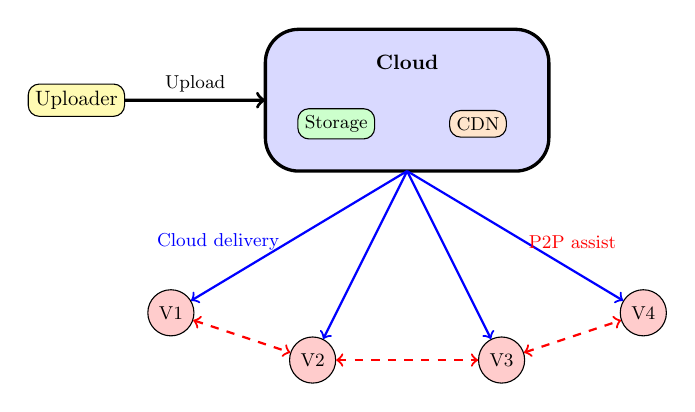
\begin{tikzpicture}[scale=0.6, every node/.style={scale=0.75}]
            % Cloud
            \draw[fill=blue!15, very thick, rounded corners=12pt] (4,5) rectangle (10,8);
            \node at (7,7.3) {\textbf{Cloud}};
            \node[draw, fill=green!20, rounded corners] at (5.5,6) {\small Storage};
            \node[draw, fill=orange!20, rounded corners] at (8.5,6) {\small CDN};
            
            % Uploader
            \node[draw, fill=yellow!30, rounded corners] (up) at (0,6.5) {Uploader};
            \draw[->, very thick] (up) -- (4,6.5) node[midway, above] {\small Upload};
            
            % Viewers
            \node[draw, fill=red!20, circle] (v1) at (2,2) {\small V1};
            \node[draw, fill=red!20, circle] (v2) at (5,1) {\small V2};
            \node[draw, fill=red!20, circle] (v3) at (9,1) {\small V3};
            \node[draw, fill=red!20, circle] (v4) at (12,2) {\small V4};
            
            % Cloud to viewers
            \draw[->, thick, blue] (7,5) -- (v1);
            \draw[->, thick, blue] (7,5) -- (v2);
            \draw[->, thick, blue] (7,5) -- (v3);
            \draw[->, thick, blue] (7,5) -- (v4);
            
            % P2P connections
            \draw[<->, thick, red, dashed] (v1) -- (v2);
            \draw[<->, thick, red, dashed] (v2) -- (v3);
            \draw[<->, thick, red, dashed] (v3) -- (v4);
            
            % Legend
            \node[blue] at (3,3.5) {\small Cloud delivery};
            \node[red] at (10.5,3.5) {\small P2P assist};
        \end{tikzpicture}
    \end{center}
    
    \vspace{0.2cm}
    \textbf{Key insight (Niu et al., 2011):} Combining cloud delivery with peer-to-peer sharing reduces cloud bandwidth costs while maintaining quality.
\end{frame}

\begin{frame}{On-Demand Video Streaming from Cloud}
    \textbf{How cloud-based VoD (Video on Demand) works:}
    
    \vspace{0.3cm}
    \begin{enumerate}
        \item \textbf{Ingest:} Content uploaded and stored in cloud
        \item \textbf{Transcode:} Video encoded at multiple bitrates/resolutions
        \item \textbf{Segment:} Video split into small chunks (2--10 seconds)
        \item \textbf{Distribute:} Chunks pushed to CDN edge servers
        \item \textbf{Stream:} Client requests chunks adaptively (DASH/HLS)
    \end{enumerate}
    
    \vspace{0.3cm}
    \begin{block}{Adaptive Bitrate Streaming (ABR)}
        Client monitors network conditions and switches between quality levels:
        \begin{itemize}
            \item Good network $\rightarrow$ 4K (25 Mbps)
            \item Medium network $\rightarrow$ 1080p (5 Mbps)
            \item Poor network $\rightarrow$ 480p (1 Mbps)
        \end{itemize}
        Seamless quality transitions without buffering!
    \end{block}
\end{frame}

\begin{frame}{P2P-Assisted Cloud Delivery}
    \textbf{Why add P2P to cloud? (Huang et al., 2008; Xu et al., 2010)}
    
    \vspace{0.3cm}
    \begin{columns}
        \begin{column}{0.5\textwidth}
            \textbf{Cloud-only problems:}
            \begin{itemize}
                \item Bandwidth cost grows linearly with users
                \item Flash crowds overwhelm servers
                \item Popular content = expensive
            \end{itemize}
            
            \vspace{0.3cm}
            \textbf{P2P advantages:}
            \begin{itemize}
                \item Users share with each other
                \item More users = more capacity
                \item Reduces cloud bandwidth by 60--80\%
            \end{itemize}
        \end{column}
        \begin{column}{0.5\textwidth}
            \textbf{Hybrid model:}
            \begin{itemize}
                \item Cloud provides base quality guarantee
                \item P2P supplements for popular content
                \item Cloud handles unpopular ``long tail''
                \item Best of both worlds
            \end{itemize}
            
            \vspace{0.3cm}
            \begin{alertblock}{Real Example}
                Systems like PPVA (Xu et al., 2010) use P2P to accelerate interactive online video sharing, reducing server load significantly.
            \end{alertblock}
        \end{column}
    \end{columns}
\end{frame}

%==============================================================================
\section{Computation Offloading for Multimedia}
%==============================================================================

\begin{frame}{The Mobile Multimedia Problem}
    \begin{alertblock}{The Dilemma}
        Mobile devices are powerful consumers of multimedia but weak producers and processors of it.
    \end{alertblock}
    
    \vspace{0.3cm}
    \begin{columns}
        \begin{column}{0.5\textwidth}
            \textbf{Mobile limitations:}
            \begin{itemize}
                \item Limited CPU/GPU power
                \item Limited battery life
                \item Limited memory
                \item Thermal constraints
            \end{itemize}
        \end{column}
        \begin{column}{0.5\textwidth}
            \textbf{Multimedia demands:}
            \begin{itemize}
                \item Video encoding is CPU-intensive
                \item AR/VR needs real-time rendering
                \item AI inference (face detection, etc.)
                \item High-quality image processing
            \end{itemize}
        \end{column}
    \end{columns}
    
    \vspace{0.3cm}
    \begin{block}{Solution: Computation Offloading}
        Send heavy computation to the cloud, get results back!
        
        (Liu et al., 2013; Ma et al., 2013)
    \end{block}
\end{frame}

\begin{frame}{What is Computation Offloading?}
    \begin{block}{Definition}
        Computation offloading is the transfer of resource-intensive computational tasks from a mobile device to external, more powerful computing platforms (cloud or edge servers).
    \end{block}
    
    \vspace{0.3cm}
    \begin{center}
        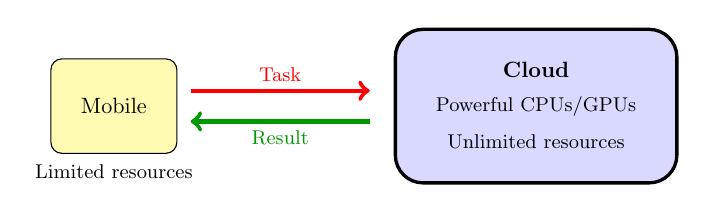
\begin{tikzpicture}[scale=0.65, every node/.style={scale=0.8}]
            % Mobile
            \node[draw, fill=yellow!30, rounded corners, minimum width=2cm, minimum height=1.5cm] (mob) at (0,0) {Mobile};
            \node[below] at (0,-1) {\small Limited resources};
            
            % Arrow
            \draw[->, ultra thick, red] (1.5,0.3) -- (5,0.3) node[midway, above] {\small Task};
            \draw[<-, ultra thick, green!60!black] (1.5,-0.3) -- (5,-0.3) node[midway, below] {\small Result};
            
            % Cloud
            \draw[fill=blue!15, very thick, rounded corners=10pt] (5.5,-1.5) rectangle (11,1.5);
            \node at (8.25,0.7) {\textbf{Cloud}};
            \node at (8.25,0) {\small Powerful CPUs/GPUs};
            \node at (8.25,-0.7) {\small Unlimited resources};
        \end{tikzpicture}
    \end{center}
    
    \vspace{0.2cm}
    \textbf{Key question:} When should we offload? Not always beneficial!
\end{frame}

\begin{frame}{When to Offload? The Decision}
    \textbf{Offloading is beneficial when (Kumar \& Lu, 2010):}
    
    \vspace{0.3cm}
    \begin{center}
        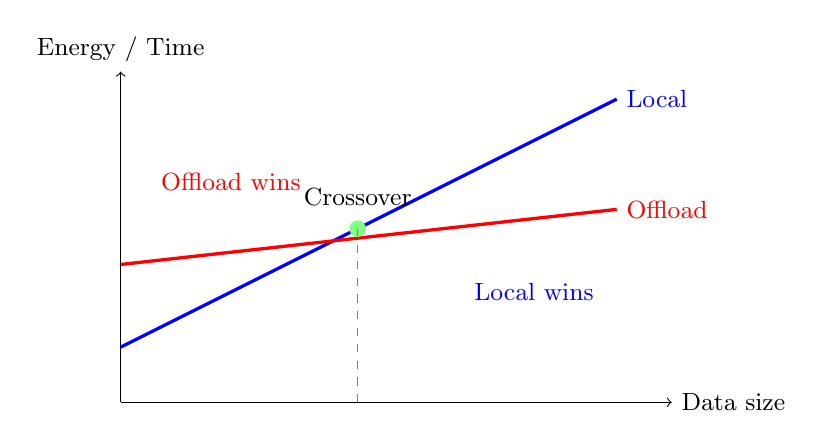
\begin{tikzpicture}[scale=0.7]
            \draw[->] (0,0) -- (10,0) node[right] {\small Data size};
            \draw[->] (0,0) -- (0,6) node[above] {\small Energy / Time};
            
            % Local execution
            \draw[blue, very thick] (0,1) -- (9,5.5);
            \node[blue, right] at (9,5.5) {\small Local};
            
            % Offload execution
            \draw[red, very thick] (0,2.5) -- (9,3.5);
            \node[red, right] at (9,3.5) {\small Offload};
            
            % Crossover
            \fill[green!50] (4.3,3.15) circle (0.15);
            \node[above] at (4.3,3.4) {\small Crossover};
            
            % Regions
            \node[red] at (2,4) {\small Offload wins};
            \node[blue] at (7.5,2) {\small Local wins};
            
            \draw[dashed, gray] (4.3,0) -- (4.3,3.15);
        \end{tikzpicture}
    \end{center}
    
    \vspace{0.2cm}
    \textbf{Offload when:} Computation is heavy but data transfer is small.
    
    \textbf{Don't offload when:} Data is huge but computation is light.
\end{frame}

\begin{frame}{Offloading Approaches}
    \textbf{Three main approaches from the literature:}
    
    \vspace{0.3cm}
    \begin{columns}
        \begin{column}{0.33\textwidth}
            \textbf{1. Full Offloading}
            
            (Cuervo et al., 2010 --- MAUI)
            \begin{itemize}
                \item Send entire task to cloud
                \item Simple to implement
                \item High latency
                \item All-or-nothing
            \end{itemize}
        \end{column}
        \begin{column}{0.33\textwidth}
            \textbf{2. Partial Offloading}
            
            (Chun et al., 2011 --- CloneCloud)
            \begin{itemize}
                \item Split task into parts
                \item Some local, some cloud
                \item Better optimization
                \item More complex
            \end{itemize}
        \end{column}
        \begin{column}{0.33\textwidth}
            \textbf{3. Adaptive Offloading}
            
            (Kumar et al., 2013)
            \begin{itemize}
                \item Decide at runtime
                \item Based on network, battery, load
                \item Best performance
                \item Most complex
            \end{itemize}
        \end{column}
    \end{columns}
\end{frame}

\begin{frame}{Multimedia Offloading Example: Video Encoding}
    \textbf{Cloud-Assisted Motion Estimation (Zhao et al., 2012 --- CAME)}
    
    \vspace{0.3cm}
    \begin{center}
        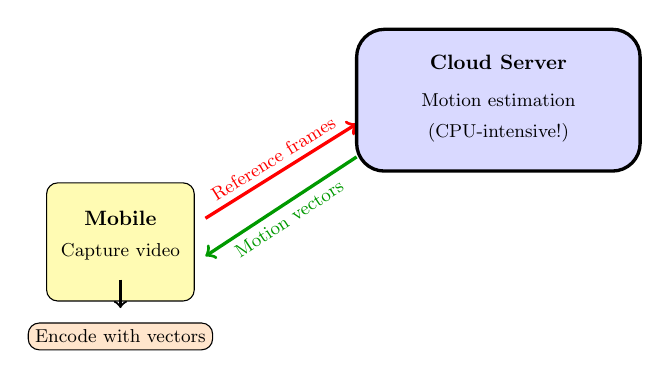
\begin{tikzpicture}[scale=0.6, every node/.style={scale=0.75}]
            % Mobile
            \node[draw, fill=yellow!30, rounded corners, minimum width=2.5cm, minimum height=2cm] (mob) at (0,0) {};
            \node at (0,0.5) {\textbf{Mobile}};
            \node at (0,-0.2) {\small Capture video};
            
            % Arrow up
            \draw[->, very thick, red] (1.8,0.5) -- (5,2.5) node[midway, above, sloped] {\small Reference frames};
            
            % Cloud
            \draw[fill=blue!15, very thick, rounded corners=10pt] (5,1.5) rectangle (11,4.5);
            \node at (8,3.8) {\textbf{Cloud Server}};
            \node at (8,3) {\small Motion estimation};
            \node at (8,2.3) {\small (CPU-intensive!)};
            
            % Arrow down
            \draw[->, very thick, green!60!black] (5,1.8) -- (1.8,-0.3) node[midway, below, sloped] {\small Motion vectors};
            
            % Mobile continues
            \node[draw, fill=orange!20, rounded corners] at (0,-2) {\small Encode with vectors};
            \draw[->, thick] (0,-0.8) -- (0,-1.4);
        \end{tikzpicture}
    \end{center}
    
    \vspace{0.2cm}
    \textbf{Result:} Mobile device saves 80\%+ of encoding energy by offloading the most expensive step (motion estimation) to the cloud.
\end{frame}

\begin{frame}{Edge Computing: Bringing Cloud Closer}
    \textbf{Problem with cloud offloading:} Latency to distant data centers.
    
    \vspace{0.3cm}
    \begin{center}
        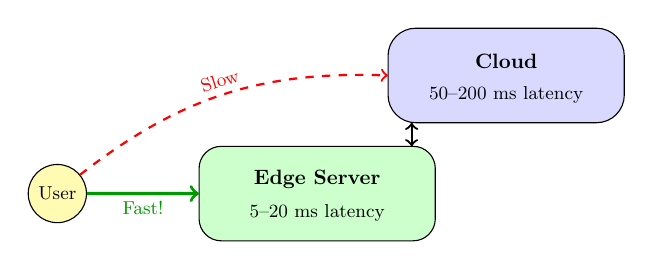
\begin{tikzpicture}[scale=0.6, every node/.style={scale=0.75}]
            % Cloud (far)
            \draw[fill=blue!15, rounded corners=10pt] (8,5) rectangle (13,7);
            \node at (10.5,6.3) {\textbf{Cloud}};
            \node at (10.5,5.6) {\small 50--200 ms latency};
            
            % Edge (near)
            \draw[fill=green!20, rounded corners=8pt] (4,2.5) rectangle (9,4.5);
            \node at (6.5,3.8) {\textbf{Edge Server}};
            \node at (6.5,3.1) {\small 5--20 ms latency};
            
            % User
            \node[draw, fill=yellow!30, circle] (user) at (1,3.5) {\small User};
            
            % Connections
            \draw[->, thick, red, dashed] (user) to[bend left=20] node[midway, above, sloped] {\small Slow} (8,6);
            \draw[->, very thick, green!60!black] (user) -- (4,3.5) node[midway, below] {\small Fast!};
            
            % Edge to cloud
            \draw[<->, thick] (8.5,4.5) -- (8.5,5);
        \end{tikzpicture}
    \end{center}
    
    \vspace{0.2cm}
    \textbf{Edge computing} places compute resources at the network edge (cell towers, ISP nodes) for ultra-low latency --- critical for AR/VR and interactive multimedia.
\end{frame}

%==============================================================================
\section{Interactive Cloud Gaming}
%==============================================================================

\begin{frame}{What is Cloud Gaming?}
    \begin{block}{Definition (Shea et al., 2013)}
        Cloud gaming renders game scenes on powerful cloud servers and streams the resulting video to thin clients. User inputs are sent back to the server.
    \end{block}
    
    \vspace{0.3cm}
    \begin{center}
        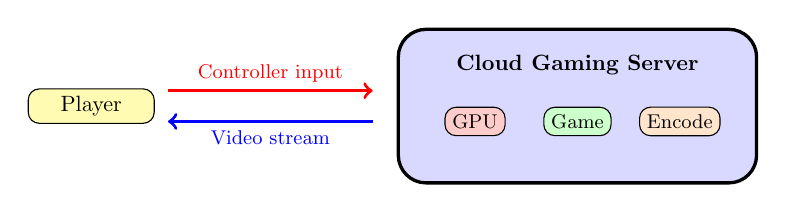
\begin{tikzpicture}[scale=0.65, every node/.style={scale=0.8}]
            % Player
            \node[draw, fill=yellow!30, rounded corners, minimum width=2cm] (player) at (0,0) {Player};
            
            % Arrows
            \draw[->, very thick, red] (1.5,0.3) -- (5.5,0.3) node[midway, above] {\small Controller input};
            \draw[<-, very thick, blue] (1.5,-0.3) -- (5.5,-0.3) node[midway, below] {\small Video stream};
            
            % Cloud
            \draw[fill=blue!15, very thick, rounded corners=10pt] (6,-1.5) rectangle (13,1.5);
            \node at (9.5,0.8) {\textbf{Cloud Gaming Server}};
            \node[draw, fill=red!20, rounded corners] at (7.5,-0.3) {\small GPU};
            \node[draw, fill=green!20, rounded corners] at (9.5,-0.3) {\small Game};
            \node[draw, fill=orange!20, rounded corners] at (11.5,-0.3) {\small Encode};
        \end{tikzpicture}
    \end{center}
    
    \vspace{0.2cm}
    \textbf{Examples:} NVIDIA GeForce NOW, Xbox Cloud Gaming, PlayStation Now, Google Stadia (discontinued)
\end{frame}

\begin{frame}{Cloud Gaming Architecture}
    \begin{center}
        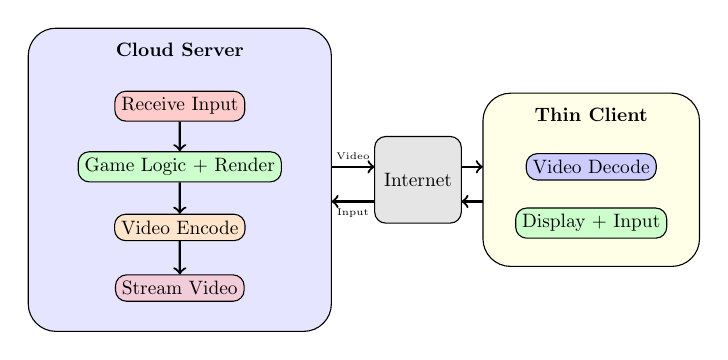
\begin{tikzpicture}[scale=0.55, every node/.style={scale=0.7}]
            % Server side
            \draw[fill=blue!10, rounded corners=10pt] (0,0) rectangle (7,7);
            \node at (3.5,6.5) {\textbf{Cloud Server}};
            
            \node[draw, fill=red!20, rounded corners, minimum width=2cm] (input) at (3.5,5.2) {Receive Input};
            \node[draw, fill=green!20, rounded corners, minimum width=2cm] (game) at (3.5,3.8) {Game Logic + Render};
            \node[draw, fill=orange!20, rounded corners, minimum width=2cm] (encode) at (3.5,2.4) {Video Encode};
            \node[draw, fill=purple!20, rounded corners, minimum width=2cm] (send) at (3.5,1) {Stream Video};
            
            \draw[->, thick] (input) -- (game);
            \draw[->, thick] (game) -- (encode);
            \draw[->, thick] (encode) -- (send);
            
            % Network
            \draw[fill=gray!20, rounded corners] (8,2.5) rectangle (10,4.5);
            \node at (9,3.5) {Internet};
            
            \draw[->, thick] (7,3.8) -- (8,3.8) node[midway, above] {\tiny Video};
            \draw[<-, thick] (7,3) -- (8,3) node[midway, below] {\tiny Input};
            
            % Client side
            \draw[fill=yellow!10, rounded corners=10pt] (10.5,1.5) rectangle (15.5,5.5);
            \node at (13,5) {\textbf{Thin Client}};
            
            \node[draw, fill=blue!20, rounded corners] at (13,3.8) {Video Decode};
            \node[draw, fill=green!20, rounded corners] at (13,2.5) {Display + Input};
            
            \draw[->, thick] (10,3.8) -- (10.5,3.8);
            \draw[<-, thick] (10,3) -- (10.5,3);
        \end{tikzpicture}
    \end{center}
    
    \vspace{0.2cm}
    \textbf{All heavy lifting happens in the cloud.} The client only decodes video and captures input.
\end{frame}

\begin{frame}{The Latency Challenge}
    \textbf{Cloud gaming's biggest enemy: LATENCY}
    
    \vspace{0.3cm}
    \begin{block}{Interaction Latency Breakdown (Chen et al., 2011)}
        \begin{center}
            \begin{tabular}{l|c}
                \toprule
                \textbf{Component} & \textbf{Typical Delay} \\
                \midrule
                Input capture \& send & 5--10 ms \\
                Network (to server) & 10--50 ms \\
                Game processing \& render & 10--30 ms \\
                Video encoding & 5--15 ms \\
                Network (to client) & 10--50 ms \\
                Video decoding \& display & 5--15 ms \\
                \midrule
                \textbf{Total round-trip} & \textbf{45--170 ms} \\
                \bottomrule
            \end{tabular}
        \end{center}
    \end{block}
    
    \vspace{0.2cm}
    \textbf{Acceptable latency (Claypool \& Claypool, 2006, 2010):}
    \begin{itemize}
        \item FPS games: $<$ 100 ms (very strict)
        \item Racing games: $<$ 150 ms
        \item Strategy games: $<$ 500 ms (more tolerant)
    \end{itemize}
\end{frame}

\begin{frame}{Cloud Gaming: Quality Challenges}
    \begin{columns}
        \begin{column}{0.5\textwidth}
            \textbf{Video Quality Issues:}
            \begin{itemize}
                \item Compression artifacts (blocking, blurring)
                \item Fast motion = harder to encode
                \item Dark scenes lose detail
                \item Resolution limited by bandwidth
            \end{itemize}
            
            \vspace{0.3cm}
            \textbf{Quality Metrics:}
            \begin{itemize}
                \item PSNR (Peak Signal-to-Noise Ratio)
                \item SSIM (Structural Similarity)
                \item MOS (Mean Opinion Score)
            \end{itemize}
        \end{column}
        \begin{column}{0.5\textwidth}
            \textbf{Typical Requirements:}
            \begin{center}
                \begin{tabular}{l|c}
                    \toprule
                    Quality & Bandwidth \\
                    \midrule
                    720p 30fps & 5 Mbps \\
                    1080p 60fps & 15 Mbps \\
                    4K 60fps & 35 Mbps \\
                    \bottomrule
                \end{tabular}
            \end{center}
            
            \vspace{0.3cm}
            \begin{alertblock}{Tradeoff}
                Higher quality $\rightarrow$ more bandwidth $\rightarrow$ more latency from encoding.
                
                Cloud gaming must balance all three!
            \end{alertblock}
        \end{column}
    \end{columns}
\end{frame}

\begin{frame}{GPU Virtualization for Cloud Gaming}
    \textbf{How to serve many gamers from one server? (Zhao et al., 2012)}
    
    \vspace{0.3cm}
    \begin{center}
        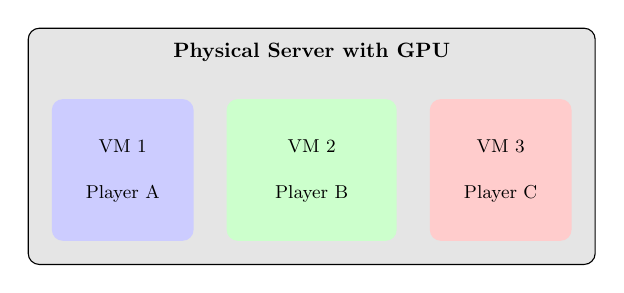
\begin{tikzpicture}[scale=0.6, every node/.style={scale=0.75}]
            % Physical server
            \draw[fill=gray!20, rounded corners] (0,0) rectangle (12,5);
            \node at (6,4.5) {\textbf{Physical Server with GPU}};
            
            % VMs
            \fill[blue!20, rounded corners] (0.5,0.5) rectangle (3.5,3.5);
            \node at (2,2.5) {\small VM 1};
            \node at (2,1.5) {\small Player A};
            
            \fill[green!20, rounded corners] (4.2,0.5) rectangle (7.8,3.5);
            \node at (6,2.5) {\small VM 2};
            \node at (6,1.5) {\small Player B};
            
            \fill[red!20, rounded corners] (8.5,0.5) rectangle (11.5,3.5);
            \node at (10,2.5) {\small VM 3};
            \node at (10,1.5) {\small Player C};
        \end{tikzpicture}
    \end{center}
    
    \vspace{0.3cm}
    \textbf{GPU virtualization} allows multiple game instances to share one physical GPU:
    \begin{itemize}
        \item Each player gets a virtual GPU slice
        \item Hardware encoding (NVENC/VCE) for low-latency video
        \item One server can host 10--30+ game sessions
    \end{itemize}
\end{frame}


%==============================================================================
\section{Case Study: Netflix}
%==============================================================================

\begin{frame}{Netflix: The World's Largest Multimedia Cloud}
    \begin{columns}
        \begin{column}{0.5\textwidth}
            \textbf{Netflix by the numbers:}
            \begin{itemize}
                \item 260+ million subscribers
                \item 190+ countries
                \item 15,000+ titles
                \item 15\%+ of global internet traffic
                \item Billions of hours streamed/month
            \end{itemize}
        \end{column}
        \begin{column}{0.5\textwidth}
            \begin{block}{The Challenge}
                How do you deliver high-quality video to 260 million people simultaneously, across every device, in every country?
            \end{block}
            
            \vspace{0.3cm}
            \textbf{Answer:} A sophisticated cloud + CDN architecture that touches every concept we've discussed.
        \end{column}
    \end{columns}
\end{frame}

\begin{frame}{Netflix Architecture: Two Brains}
    \begin{center}
        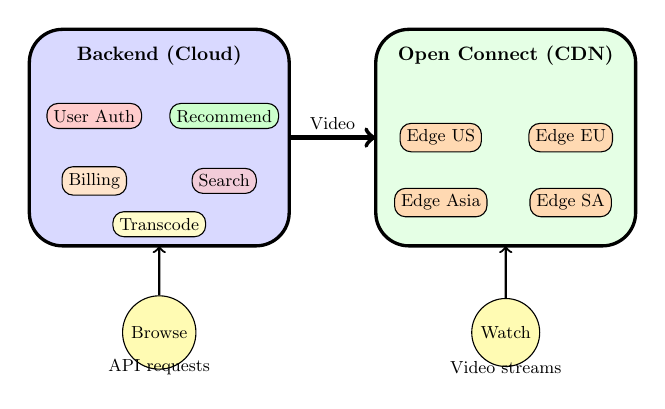
\begin{tikzpicture}[scale=0.55, every node/.style={scale=0.7}]
            % Backend Cloud
            \draw[fill=blue!15, very thick, rounded corners=12pt] (0,3) rectangle (6,8);
            \node at (3,7.4) {\textbf{Backend (Cloud)}};
            \node[draw, fill=red!20, rounded corners] at (1.5,6) {\small User Auth};
            \node[draw, fill=green!20, rounded corners] at (4.5,6) {\small Recommend};
            \node[draw, fill=orange!20, rounded corners] at (1.5,4.5) {\small Billing};
            \node[draw, fill=purple!20, rounded corners] at (4.5,4.5) {\small Search};
            \node[draw, fill=yellow!20, rounded corners] at (3,3.5) {\small Transcode};
            
            % CDN
            \draw[fill=green!10, very thick, rounded corners=12pt] (8,3) rectangle (14,8);
            \node at (11,7.4) {\textbf{Open Connect (CDN)}};
            
            % Edge servers
            \node[draw, fill=orange!30, rounded corners] at (9.5,5.5) {\small Edge US};
            \node[draw, fill=orange!30, rounded corners] at (12.5,5.5) {\small Edge EU};
            \node[draw, fill=orange!30, rounded corners] at (9.5,4) {\small Edge Asia};
            \node[draw, fill=orange!30, rounded corners] at (12.5,4) {\small Edge SA};
            
            % Arrow between
            \draw[->, ultra thick] (6,5.5) -- (8,5.5) node[midway, above] {\small Video};
            
            % Users
            \node[draw, fill=yellow!30, circle] (u1) at (3,1) {\small Browse};
            \node[draw, fill=yellow!30, circle] (u2) at (11,1) {\small Watch};
            
            \draw[->, thick] (u1) -- (3,3);
            \draw[->, thick] (u2) -- (11,3);
            
            % Labels
            \node at (3,0.2) {\small API requests};
            \node at (11,0.2) {\small Video streams};
        \end{tikzpicture}
    \end{center}
    
    \vspace{0.2cm}
    \textbf{Two separate systems:}
    \begin{itemize}
        \item \textbf{Backend (Cloud):} Handles everything except video streaming --- user accounts, recommendations, search, billing, transcoding
        \item \textbf{Open Connect (CDN):} Handles only video delivery --- distributed edge servers worldwide
    \end{itemize}
\end{frame}

\begin{frame}{Netflix: Cloud Computing (Backend)}
    \textbf{Netflix uses cloud for all non-streaming operations:}
    
    \vspace{0.3cm}
    \begin{columns}
        \begin{column}{0.5\textwidth}
            \textbf{Microservices Architecture:}
            \begin{itemize}
                \item 1000+ microservices
                \item Each handles one function
                \item Independent scaling
                \item Fault isolation
            \end{itemize}
            
            \vspace{0.3cm}
            \textbf{Why microservices?}
            
            A 2008 database corruption caused a 3-day outage. Netflix migrated to microservices over 8 years to prevent this.
        \end{column}
        \begin{column}{0.5\textwidth}
            \textbf{Key cloud services used:}
            \begin{itemize}
                \item \textbf{Compute:} Thousands of virtual servers
                \item \textbf{Storage:} Petabytes of video content
                \item \textbf{Database:} User data, viewing history
                \item \textbf{ML/AI:} Recommendation engine
                \item \textbf{Analytics:} Real-time monitoring
            \end{itemize}
            
            \vspace{0.3cm}
            \begin{block}{Scale}
                Netflix handles millions of API requests per second from its cloud backend.
            \end{block}
        \end{column}
    \end{columns}
\end{frame}

\begin{frame}{Netflix: Video Processing Pipeline}
    \textbf{From studio master to your screen:}
    
    \vspace{0.3cm}
    \begin{center}
        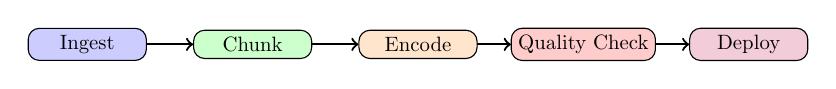
\begin{tikzpicture}[scale=0.6, every node/.style={scale=0.75}]
            \node[draw, fill=blue!20, rounded corners, minimum width=2cm] (ingest) at (0,0) {Ingest};
            \node[draw, fill=green!20, rounded corners, minimum width=2cm] (chunk) at (3.5,0) {Chunk};
            \node[draw, fill=orange!20, rounded corners, minimum width=2cm] (encode) at (7,0) {Encode};
            \node[draw, fill=red!20, rounded corners, minimum width=2cm] (quality) at (10.5,0) {Quality Check};
            \node[draw, fill=purple!20, rounded corners, minimum width=2cm] (deploy) at (14,0) {Deploy};
            
            \draw[->, thick] (ingest) -- (chunk);
            \draw[->, thick] (chunk) -- (encode);
            \draw[->, thick] (encode) -- (quality);
            \draw[->, thick] (quality) -- (deploy);
        \end{tikzpicture}
    \end{center}
    
    \vspace{0.3cm}
    \begin{enumerate}
        \item \textbf{Ingest:} Receive studio master (huge, uncompressed)
        \item \textbf{Chunk:} Split into small segments for parallel processing
        \item \textbf{Encode:} Transcode into 100+ versions (different resolutions, bitrates, codecs)
        \item \textbf{Quality Check:} VMAF score ensures quality meets standards
        \item \textbf{Deploy:} Push to Open Connect CDN servers worldwide
    \end{enumerate}
    
    \vspace{0.2cm}
    \textit{One movie generates over 100 encoded versions using hundreds of cloud instances in parallel!}
\end{frame}

\begin{frame}{Netflix: Per-Title Encoding}
    \textbf{Not all content is equal:}
    
    \vspace{0.3cm}
    \begin{columns}
        \begin{column}{0.5\textwidth}
            \textbf{Simple content} (e.g., animated show):
            \begin{itemize}
                \item Flat colors, simple motion
                \item Looks great at low bitrate
                \item 1080p at 2 Mbps is fine
            \end{itemize}
            
            \vspace{0.3cm}
            \textbf{Complex content} (e.g., action movie):
            \begin{itemize}
                \item Fast motion, explosions, detail
                \item Needs higher bitrate
                \item 1080p needs 8+ Mbps
            \end{itemize}
        \end{column}
        \begin{column}{0.5\textwidth}
            \begin{block}{Per-Title Encoding}
                Netflix analyzes each title's complexity and creates a custom encoding ladder:
                \begin{itemize}
                    \item Simple content: fewer, lower bitrate versions
                    \item Complex content: more, higher bitrate versions
                \end{itemize}
                
                \vspace{0.2cm}
                \textbf{Result:} 20\% bandwidth savings with same perceived quality!
            \end{block}
            
            \vspace{0.2cm}
            \textit{Uses VMAF (Video Multi-Method Assessment Fusion) to measure perceptual quality.}
        \end{column}
    \end{columns}
\end{frame}

\begin{frame}{Netflix: Open Connect CDN}
    \textbf{Netflix built its own CDN instead of renting one:}
    
    \vspace{0.3cm}
    \begin{columns}
        \begin{column}{0.5\textwidth}
            \textbf{How Open Connect works:}
            \begin{itemize}
                \item Custom hardware appliances (OCAs)
                \item Placed inside ISP networks
                \item Pre-loaded with popular content
                \item Serve video from local network
            \end{itemize}
            
            \vspace{0.3cm}
            \textbf{Scale:}
            \begin{itemize}
                \item 17,000+ servers
                \item 6,000+ ISP partners
                \item 190+ countries
                \item Handles all video traffic
            \end{itemize}
        \end{column}
        \begin{column}{0.5\textwidth}
            \begin{center}
                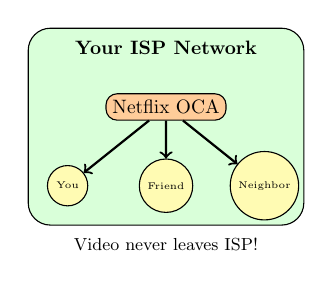
\begin{tikzpicture}[scale=0.5, every node/.style={scale=0.7}]
                    % ISP
                    \draw[fill=green!15, rounded corners=8pt] (0,0) rectangle (7,5);
                    \node at (3.5,4.5) {\textbf{Your ISP Network}};
                    
                    % OCA
                    \node[draw, fill=orange!40, rounded corners, minimum width=2cm] (oca) at (3.5,3) {Netflix OCA};
                    
                    % Users
                    \node[draw, fill=yellow!30, circle] (u1) at (1,1) {\tiny You};
                    \node[draw, fill=yellow!30, circle] (u2) at (3.5,1) {\tiny Friend};
                    \node[draw, fill=yellow!30, circle] (u3) at (6,1) {\tiny Neighbor};
                    
                    \draw[->, thick] (oca) -- (u1);
                    \draw[->, thick] (oca) -- (u2);
                    \draw[->, thick] (oca) -- (u3);
                    
                    \node at (3.5,-0.5) {\small Video never leaves ISP!};
                \end{tikzpicture}
            \end{center}
            
            \vspace{0.2cm}
            \begin{alertblock}{Key Benefit}
                Video is served from inside your ISP --- minimal latency, no internet congestion!
            \end{alertblock}
        \end{column}
    \end{columns}
\end{frame}

\begin{frame}{Netflix: Adaptive Streaming}
    \textbf{Netflix adapts quality in real-time:}
    
    \vspace{0.3cm}
    \begin{center}
        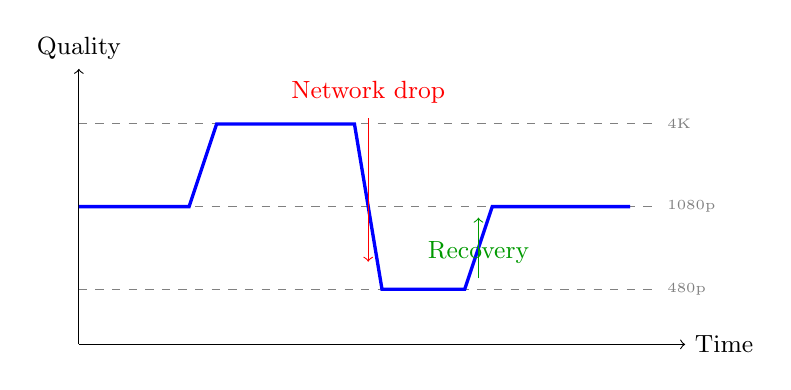
\begin{tikzpicture}[scale=0.7]
            \draw[->] (0,0) -- (11,0) node[right] {\small Time};
            \draw[->] (0,0) -- (0,5) node[above] {\small Quality};
            
            % Quality levels
            \draw[dashed, gray] (0,1) -- (10.5,1) node[right] {\tiny 480p};
            \draw[dashed, gray] (0,2.5) -- (10.5,2.5) node[right] {\tiny 1080p};
            \draw[dashed, gray] (0,4) -- (10.5,4) node[right] {\tiny 4K};
            
            % Adaptive line
            \draw[blue, very thick] (0,2.5) -- (2,2.5) -- (2.5,4) -- (5,4) -- (5.5,1) -- (7,1) -- (7.5,2.5) -- (10,2.5);
            
            % Annotations
            \node[above, red] at (5.25,4.2) {\small Network drop};
            \draw[->, red] (5.25,4.1) -- (5.25,1.5);
            
            \node[above, green!60!black] at (7.25,1.3) {\small Recovery};
            \draw[->, green!60!black] (7.25,1.2) -- (7.25,2.3);
        \end{tikzpicture}
    \end{center}
    
    \vspace{0.2cm}
    \textbf{How it works:}
    \begin{itemize}
        \item Client measures download speed every few seconds
        \item Requests next chunk at appropriate quality
        \item Maintains buffer to absorb short network dips
        \item Goal: maximize quality while avoiding rebuffering
    \end{itemize}
\end{frame}

\begin{frame}{Netflix: Putting It All Together}
    \textbf{What happens when you press ``Play'':}
    
    \vspace{0.3cm}
    \begin{enumerate}
        \item \textbf{Your app} contacts Netflix backend (cloud) for authentication
        \item \textbf{Backend} checks your subscription, selects content
        \item \textbf{Recommendation engine} (cloud ML) suggested this title
        \item \textbf{Backend} determines best Open Connect server near you
        \item \textbf{Your app} connects to nearest OCA (inside your ISP)
        \item \textbf{OCA} starts streaming pre-encoded video chunks
        \item \textbf{Your app} adapts quality based on network conditions
        \item \textbf{Backend} logs viewing data for future recommendations
    \end{enumerate}
    
    \vspace{0.3cm}
    \begin{block}{All Concepts in Action}
        Cloud computing (backend) + Cloud storage (content) + CDN (delivery) + Adaptive streaming (quality) + ML/AI (recommendations)
    \end{block}
\end{frame}

\begin{frame}{Netflix: Lessons for Multimedia Cloud}
    \begin{columns}
        \begin{column}{0.5\textwidth}
            \textbf{What Netflix teaches us:}
            \begin{enumerate}
                \item \textbf{Separate concerns:} Backend logic vs content delivery
                \item \textbf{Build your own CDN} if scale justifies it
                \item \textbf{Per-title optimization} beats one-size-fits-all
                \item \textbf{Adaptive streaming} is essential
                \item \textbf{Microservices} enable independent scaling
            \end{enumerate}
        \end{column}
        \begin{column}{0.5\textwidth}
            \textbf{Connecting to textbook concepts:}
            \begin{itemize}
                \item \textbf{Cloud overview:} Netflix uses all three service models
                \item \textbf{Media sharing:} Open Connect = cloud-assisted delivery
                \item \textbf{Offloading:} Transcoding offloaded to cloud
                \item \textbf{QoE:} VMAF-driven encoding quality
            \end{itemize}
            
            \vspace{0.3cm}
            \begin{alertblock}{Key Takeaway}
                Netflix is a textbook example of every multimedia cloud concept working together at massive scale.
            \end{alertblock}
        \end{column}
    \end{columns}
\end{frame}

%==============================================================================
\section{Summary}
%==============================================================================

\begin{frame}{Key Takeaways}
    \begin{enumerate}
        \item \textbf{Cloud computing} provides on-demand, elastic resources (IaaS, PaaS, SaaS) ideal for multimedia's heavy demands
        
        \item \textbf{Multimedia cloud computing} combines cloud storage, processing, delivery, and analytics for media services
        
        \item \textbf{Cloud-assisted media sharing} uses hybrid cloud + P2P architectures to reduce cost while maintaining quality
        
        \item \textbf{Computation offloading} moves heavy tasks (encoding, rendering) from mobile devices to cloud/edge servers
        
        \item \textbf{Interactive cloud gaming} streams rendered video from cloud GPUs, with latency as the critical challenge
        
        \item \textbf{Netflix} demonstrates all these concepts at scale: cloud backend, custom CDN, per-title encoding, adaptive streaming
    \end{enumerate}
\end{frame}

\begin{frame}{Key References}
    \small
    \begin{itemize}
        \item Mell \& Grance (2011). The NIST Definition of Cloud Computing. NIST SP 800-145.
        \item Zhu, Luo, Wang \& Li (2011). Multimedia Cloud Computing. \textit{IEEE Signal Processing Magazine}.
        \item Armbrust et al. (2010). A View of Cloud Computing. \textit{Communications of the ACM}.
        \item Liu et al. (2013). Gearing Resource-Poor Mobile Devices with Powerful Clouds. \textit{IEEE Wireless Communications}.
        \item Kumar \& Lu (2010). Cloud Computing for Mobile Users: Can Offloading Save Energy? \textit{IEEE Computer}.
        \item Zhao et al. (2012). CAME: Cloud-Assisted Motion Estimation. \textit{ACM NOSSDAV}.
        \item Shea, Liu, Ngai \& Cui (2013). Cloud Gaming: Architecture and Performance. \textit{IEEE Network}.
        \item Claypool \& Claypool (2006). Latency and Player Actions in Online Games. \textit{Communications of the ACM}.
    \end{itemize}
    
    \vspace{0.2cm}
    \textbf{Textbook:} Li, Drew \& Liu, \textit{Fundamentals of Multimedia}, 3rd Ed., Chapter 19.
\end{frame}

\begin{frame}
    \begin{center}
        \Huge{\textbf{Thank You!}}
        
        \vspace{1cm}
        \Large{Questions?}
        
        \vspace{1.5cm}
        \normalsize
        \textit{``The cloud is not just about technology --- it's about enabling new ways to create, share, and experience multimedia.''}
    \end{center}
\end{frame}

\end{document}
